\chapter{Méthodologie de la recherche}
\label{ch:methodo}

Une démarche classique de recherche commence par la formulation d'une question 
de départ. La question qui a initié nos travaux est la suivante~: «~Comment 
simuler afin de les valider les SI des Smart Grids ?~».  Comme en témoigne notre 
l'état de l'art, cette question fait l'objet de très peu de travaux (section 
\ref{approche_simu_existante}). Une recherche exploratoire a donc été nécessaire 
pour mettre en évidence les caractéristiques d'un phénomène nouveau selon une 
démarche inductive. 

Cette phase exploratoire a été préalable à la définition du cadre d'architecture 
\textit{ExcuteEA}. La construction de ce cadre d'architecture et sa mise à 
l'épreuve ont fait l'objet d'une recherche explicative pour laquelle nos avons 
adopté une démarche déductive.

L'intérêt de cette partie est de traiter la question de la cohérence entre nos 
objectifs de recherche et la démarche que nous adoptons pour y répondre. Mais 
nous ne cherchons pas à donner l'impression que notre plan de recherche a été 
entièrement établi avant de le mettre en œuvre. À l'inverse, nous l'avons 
construit au fur et à mesure de nos interactions avec le terrain d'étude. 

Tout d'abord, nous présentons la démarche inductive entreprise pour délimiter 
notre objet d'étude. Nous reprenons les étapes de cette recherche exploratoire 
par ordre chronologique~: exploration de la vue métier, puis de la vue 
applicative et en fin de la vue fonctionnelle. Nous présentons ensuite la 
démarche déductive ayant abouti à la construction du cadre d'architecture 
ExecuteEA.

%"Quelle que soit la nature de la démarche, la capacité d'ouverture et de prise 
%en compte d'éléments nouveaux est primordiale." ici ou dans la conclusion ?

%Dans une démarche classique de recherche, la définition de l'objet d'étude est 
%préalable à la 
%Plusieurs méthodes de recherche
%démarches de recherches employée par ordres chronologiques
%Combinaisons de méthodes 
%Vocation exploratoires de nos recherches
%Nous ne cherchons pas ici à donner l'impression que nous avons entièrement mis 
%au point notre plan de recherche avant de le mettre en œuvre. Celui-ci s'est au 
%contraire construit au fur et à mesure de notre interaction avec le terrain.
%
%"la cohérence du protocole de recherche avec la nature des questions que nous 
%nous posons"
%"Mais un autre élément mérite d'être distingué : la délimitation de l'objet 
%d'étude pose des problèmes tels qu'elle constitue une recherche en elle-même"
%"Quelle que soit la nature de la démarche, la capacité d'ouverture et de prise 
%en compte d'éléments nouveaux est primordiale."


	\section{Délimitation de l'objet de recherche}
%	Q : Est-ce que le recours à la demarche inductive est bien justifié ?
%		Est-ce l'investigation satisfait bien les critères de cohérence interne ?
		
	Une attention singulière est apportée à la délimitation de l'objet d'étude. 
Cette délimitation est souvent le résultat de l'observation du terrain d'étude~: 
l'entreprise et son SI d'une manière générale et l'entreprise et son SI dans le 
cas particulier des Smart Grids. L'entreprise et son SI forment un système 
complexe dont l'observation n'est pas triviale. La délimitation de l'objet 
d'étude a donc été en soi à l'origine d'une démarche de recherche.
	
	Cette partie a pour objectif de démonter la pertinence d'une démarche inductive 
pour l'identification de notre objet d'étude. D'une part, une démarche inductive 
est utile pour formuler des hypothèses ou soulever des questions et pour aborder 
un problème qui a été peu étudié comme c'est le cas de la simulation des SI. 
Elle aboutit à des propositions générales à partir de cas particuliers~: c'est 
une démarche par exploration. 
	Cette démarche est donc adaptée pour~: 
	\begin{enumerate}
	\item délimiter l'objet de l'étude, c'est à dire identifié ce qui est dans le 
contexte de la simulation des SI et ce qui ne l'est pas~;
	\item jeter les bases d'une étude théorique ultérieure.
	\end{enumerate}
	
	D'autre part, l'induction est une démarche de recherche classique en sciences 
sociales. Elle correspond au raisonnement empiriste qui affirme que 
l'observation et l'expérience sont la source de la connaissance du monde réel et 
du concret \cite{madeleine2001methodes}. Nous cherchons en effet à comprendre 
notre objet d'étude empiriquement. Le recours à cette démarche est d'autant plus 
justifié par la nature socio-technique du SI. En définissant le SI, Robert Reix 
met en évidence sa composante sociale (\ref{ch:EA}). 
	
	%Une étude ethnographique est Notre démarche inductive est donc doublée d'.

	La volonté d'identification de notre objet d'étude est portée par la question 
suivante «~Qu'est ce que la simulation d'un SI d'entreprise ?~». Néanmoins, même 
empirique, une démarche de recherche doit nécessairement s'inscrire dans un 
cadre de cohérence. Nous avons donc veillé à construire un protocole 
d'investigation épistémologiquement valide et conforme aux critères de cohérence 
interne. Notre protocole d'investigation est axé sur l'observation et 
l'expérience. Il est constitué de trois grandes étapes ~:
		
		\begin{enumerate}
		
	\item observation du terrain d'étude, c'est à dire analyse des pratiques 
courantes des personnes concernées par la simulation. Nous avons identifié deux 
catégories de personnes susceptibles de nous intéresser~: les experts (en SI ou 
en simulation) et les personnes susceptibles d'instrumenter la simulation des SI 
pour leurs travaux de recherche ou d'ingénierie (il s'agit là des utilisateurs 
finaux). Nous avons privilégié les ingénieurs-chercheurs d'\gls{edf}~R\&D car le 
contexte \gls{cifre} de la thèse a facilité l'accès à ces 
personnes.L'observation aboutit à la formulation d'hypothèses «~aprioristes~». 
Ce type d'hypothèse est exploratoire car elles ont pour but de soulever des 
interrogations~;
	%observatio participative, démarche ethnographique
	
	\item développement d'un prototype de simulation tenant compte du résultat des 
observations de l'étape précédente. Le prototype n'a pas pour vocation de 
proposer une solution finale mais plutôt tester rapidement les hypothèses 
formulées précédemment~;
	
	\item validation ou mise à l'épreuve du prototype sur le terrain d'étude. Cette 
mise à l'épreuve commence par la définition d'un cas d'application pertinent 
permettant de vérifier les hypothèses formulées à l'étape d'observation. Elle se 
poursuit par la collecte et l'analyse du retour des personnes concernées. Le 
contexte \gls{cifre} a là aussi facilité les échanges avec les 
ingénieurs-chercheurs de EDF R\&D, et en particulier ceux du département 
\gls{mire}. Notre intégration à l'équipe des ingénieurs-cherches du département 
\gls{mire}, et en particulier à l'équipe du projet de simulation des Smart Grid, 
a contribué à la qualité des échanges avec les personnes interrogées.
	
		\end{enumerate}
		
	Le raisonnement par induction aboutit à des propositions générales à partir de 
cas singuliers. Nous avons donc commencer par décomposer le terrain d'étude, 
c'est à dire le SI de l'entreprise. Les bases théoriques de la discipline des SI 
ont permis de procéder à cette décomposition afin de mettre en évidence ses 
singularités. Les approches par points de vue sont largement utilisée pour 
traiter la complexité des SI en le décomposant en plusieurs vues~: la vue 
métier, la vue fonctionnelle, la vue applicative, la vue technique. Chaque vue 
correspond à la perspective d'un groupe de personnes aux profils différents mais 
complémentaires. Les investigations ont été menées sur les trois premières vue — 
métier, fonctionnelle, applicative. La vue technique n'a pas été traitée~: le 
temps nécessaire aux expérimentations est incompatible avec les délais de cette 
thèse et son financement dans le cadre d'une \gls{cifre}.
	
	Le protocole d'investigation est alors appliqué à chacune des vues métier, 
fonctionnelle et applicative. L'objectif de la démarche engagée est de définir 
l'objet d'étude, en ayant comme question de départ «~Qu'est ce que la simulation 
d'un SI d'entreprise ?~». Cependant, nous avons veillé à garder une capacité 
d'ouverture aux idées nouvelles. Nous présentons
	
		\subsection{Investigations menées pour la vue métier}
			La première étape d'observation a débuté avec un stage de fin d'étude de six mois que nous avons effectué au sein du département \gls{mire}. L'objectif du stage a consisté à explorer le sujet «~~Simulation du SI des Smart Grids » afin de préparer un sujet de thèse. Il s'est donc accordé avec l'objectif des investigations menées pour la vue métier.
			
			\subsubsection{Observation}
				Pour cette première phase d'observation, des entretiens ont été menés avec des experts SI internes à l'entreprise et mais aussi externes à celle-ci lors d'un séminaire professionnel\footnote{Model Driven Day, 21 novembre 2001, Paris Cœur Défense}. Des entretiens ont aussi été menés avec des ingénieurs-chercheurs du département \gls{mire} ayant participé à des démonstrateurs Smart Grids européens pour mettre en évidence les pratiques de spécification de la composante SI des Smart Grids. 

				Les hypothèses formulées à l'issue des ces observations sont les suivantes~:
				\begin{itemize}
					\item la simulation de SI est une discipline peu étudiée~;
					\item la simulation des processus métier est pertinente pour les SI des Smart Grids dans le mesure ou elle permet de valider les scénarios élaborés pour les démonstrateurs, mais aussi pour les SI tout court~;
					\item lors de cette simulation, il est nécessaire de maintenir une cohérence entre processus et données manipulées.
				\end{itemize}
		
			\subsubsection{Prototypage}
				Le prototypage a nécessité une étude des outils existants proposant de simuler des processus métier, ce qui a permis d'identifier les outils suivant~: Enterprise Architect, Bonita, Amuse et Rhapsody. Il a ensuite essentiellement à tester leur capacité de simulation selon une grille d'évaluation. Le critère de sélection principal a été la capacité de l'outil à exécuter des diagrammes d'activité UML. En effet, c'est dans ce langage que sont représentés les processus métier dans les documents de spécification des démonstrateurs Smart Grid. Le deuxième critère d'évaluation retenu a été la possibilité d'ajout de nouvelles fonctionnalités à l'outil. À l'issue de cette étude comparative, l'outil Enterprise Architect dans sa version 9.2 a été retenu. En effet, à l'époque de l'étude, EA était le seul à pouvoir animer des diagrammes d'activité et à offrir la possibilité d'ajout de fonctionnalité par le mécanisme de plugin. C'était en outre l'outil de modélisation UML de référence de l'équipe d'ingénieurs-chercheurs au sein de laquelle nous avons effectué ce stage.
				
				Cependant, dans sa version 9.2, l'outil n'assure pas la cohérence entre les objets métier (modélisés avec diagramme de classe) et le processus (modélisé avec un diagramme d'activité) au cours de la simulation. De plus, l'outil ne gère pas la persistance des résultats de la simulation. La mise en cohérence a donc nécessité le développement d'un plugin que nous avons baptisé DataSimu. DataSimu permet de (1)~créer un jeu de donnée en entrée de la simulation à partir des concepts métier en instanciant un diagramme de classe (2)~simuler le processus métier avec ce jeu de donnée (3)~récupérer le jeu de données en sortie de la simulation et les stocker dans une base de données. Nous avons mené l'implémentation de DataSimu en binôme avec un étudiant en troisième année d'école d'ingénieur. L'interface graphique de DataSimu est illustrée par la figure. L'annexe (ANNEXE) détaille l'architecture de DataSimu et présente un manuel d'utilisation. 
				
				\begin{figure}[!ht]
 \begin{center}
  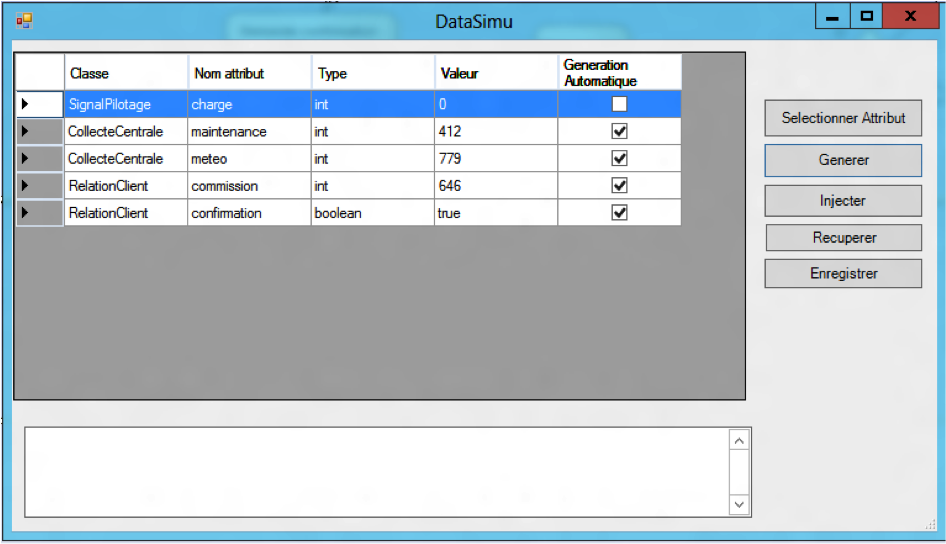
\includegraphics[width=1\textwidth]{figures/6_methodologie/data_simu.png}
 \end{center}
 \caption{Interface Graphique de DataSimu}
 \label{fig:data_simu}
\end{figure}
				
			\subsubsection{Validation}
			Pour valider les hypothèses formulées à l'issue de l'observation, un cas d'application Smart Grid a été mis au point~: le pilotage d'une charge domestique. Ce cas d'application est issu de l'étude des spécifications des démonstrateurs Smart Grid ADDRESS et PREMIO introduits dans la section~\ref{sec:DemonstrateursSG}. Il s'agit de piloter une batterie de stockage d'énergie installée chez un client (particulier ou industriel). En fonction de l'état du réseau, une centrale de pilotage contrôle cette batterie (stockage d'énergie pour une utilisation ultérieure), tout en tenant compte des consignes du client. Ce cas métier a été modélisé et simulé avec l'outil Enterprise Architect doté du plugin DataSimu. Une description détaillée du cas métier et du déroulement de la simulation est donnée dans l'annexe \ref{annexe:DataSimu}. 
			
			Le prototype de simulation et sa mise en œuvre à travers le cas métier du pilotage d'une charge domestique ont été soumis aux experts SI du département \gls{mire} et aux ingénieurs-chercheurs contribuant aux démonstrateurs Smart Grid PREMIO et ADDRESS. Les entretiens suivant la démonstration ont validé (1) la pertinence de la simulation dans le contexte des SI des Smart Grids (2) la séparation du processus métier et des objets métier tout en maintenant une cohérence lors de la simulation. 
			
			Ces entretiens, en plus de l'étude des outils de simulation des processus métier, ont permis de constater que la question de la simulation est peu abordé dans le contexte des SI. Ces travaux d'investigation ont de plus donnée lieu à une publication \cite{seghiri2012animation} et ont été poursuivis par les travaux présentés dans cette thèse. 

	
		\subsection{Investigations menées pour la vue fonctionnelle} 
			\subsubsection{Observation}
		
			\subsubsection{Prototypage}
		
			\subsubsection{Validation}
	DSML pour le Volt Var Control
		\subsection{Investigations menées pour la vue applicative} 
			\subsubsection{Observation}
		
			\subsubsection{Prototypage}
		
			\subsubsection{Validation}
	Ptolemy : Simu appli + couplage réseau élec
	
	
		\subsection{Conclusion}
Redéfinition de l'objet d'étude
Reformulation de la question de départ -> ref problématique 
Le cœur de la problématique 
Adéquation de la démarche et de l'objectif de la recherche (objet d'étude)
	
La question de l'analyse par simulation du SI fait l'objet de 
Démarche exploratoire / Démarche ethnographique 
La délimitation du sujet de recherches est en soit à l'origine d'une démarche de 
recherche à part entière  inductive, se prête mieux au sujet nouveau, faisant 
l'objet de peu de travaux
Jeter les bases d'une étude ultérieure


Mettre en évidence les caractéristiques du phénomène et construire des 
hypothèses 
"Les hypothèses et même les questions sont susceptibles d'évoluer au fur et à 
mesure de la recherche"

"En retour, le travail empirique se verra régulièrement réorienté en fonction 
des approfondissements successifs du cadre théorique "

Étude sociologique -> entretien avec les experts, sur leur avis de nos 
prototypes mais aussi 

Plusieurs démarches d'investigation 
prototypage et entretien 
ou SI transverse et SI spécialisé ? SI purement logiciel / SI socio-technique 
(interaction humaine) 
Une différence d'échelle 
		 


	\section{Conceptualisation / construction du cadre d'architecture 
\textit{ExecuteEA}}
%À partir de la compréhension empirique de notre objet d'étude et de la 
formulation d'une problématique 
La reformulation de la question de départ abouti à la définition d'une 
problématique 
La question de départ est au cœur de la problématique 

permet la Définition du cadre théorique 

La proposition est au contraire déductive
Sujet identifiés, hypothèses formulées
systèmes similaires : SI et entreprise -> établir les similarités
Les hypothèses etc.  
Choix de la théorie à appliquer : IDM (hypothèse et conclusion)/ apport de l'IDM 
a-à l'EA, hypothèse (même problématique) à une échelle différente  ‹
Itérative et là Smook 

	\subsubsection{Conclusion}
	
	
	
	
	
